\documentclass{article}
%%%%%%%%%%%%%%%%%%%%%%%%%%%%%%%%%%%%%%%%%%%%%%%%%%%%%%
% Math
%%%%%%%%%%%%%%%%%%%%%%%%%%%%%%%%%%%%%%%%%%%%%%%%%%%%%%
\usepackage{amsmath}
\usepackage{amssymb}
\usepackage{amsfonts} %para usar as fontes %matematicas, e pega fontes para \mathbb
\usepackage{amsthm}   %ambientes com teoremas (usar depois de amsmath)
%\usepackage{biblatex}
%\usepackage{natbib}

%%%%%%%%%%%%%%%%%%%%%%%%%%%%%%%%%%%%%%%%%%%%%%%%%%%%%%
%Graphs
%%%%%%%%%%%%%%%%%%%%%%%%%%%%%%%%%%%%%%%%%%%%%%%%%%%%%%
\usepackage{graphics}
\usepackage{graphicx}
\usepackage{texdraw}
\usepackage{color}
\usepackage{subfigure} 
\usepackage{tikz}
\usepackage[usenames,dvipsnames]{pstricks}
\usepackage{epsfig}
%\usepackage{pst-grad} % For gradients
%\usepackage{pst-plot} % For axes
%\usepackage{movie15}
\usepackage{animate}
\usetikzlibrary{decorations.fractals}
\usepackage{tikz}
%\usepackage{wrapfig}
\usepackage{pstricks}

%%%%%%%%%%%%%%%%%%%%%%%%%%%%%%%%%%%%%%%%%%%%%%%%%%%%%%
% Format
%%%%%%%%%%%%%%%%%%%%%%%%%%%%%%%%%%%%%%%%%%%%%%%%%%%%%%
\usepackage[figurename=Fig.]{caption}
\usepackage[labelformat=empty]{caption}
\usepackage{gensymb}
\usepackage{cancel}
\usepackage{caption} % removing prefix from figure caption in LaTeX
\usepackage{subcaption}
\usepackage{url}
\usepackage{setspace}
%\usepackage{verbatim}
\usepackage{hyperref}
\usepackage{fancyhdr}
\usepackage{verbatim}
\usepackage{pgf}
%%%%%%%%%%%%%%%%%%%%%%%%%%%%%%%%%%%%%%%%%%%%%%%%%%%%%%
% Graphs path to the Picture Folder
%%%%%%%%%%%%%%%%%%%%%%%%%%%%%%%%%%%%%%%%%%%%%%%%%%%%%%
%\graphicspath{/home/henry/Desktop/UTEP_Proposal_Thesis/PhD_Thesis/Pictures}
\graphicspath{{Pictures/}{Data/}} % Two folders Picture and Data    
%%%%%%%%%%%%%%%%%%%%%%%%%%%%%%%%%%%%%%%%%%%%%%%%%%%%%%
% page edition
%%%%%%%%%%%%%%%%%%%%%%%%%%%%%%%%%%%%%%%%%%%%%%%%%%%%%%
%\linespread{2.5}
\addtolength{\textwidth}{3cm}
\addtolength{\textheight}{3cm}
\addtolength{\hoffset}{-2cm}
% In case you need to adjust margins:
\topmargin=-0.5 in      %
\evensidemargin= .5 in     %
\oddsidemargin= .5 in      %
\textwidth = 7 in        %
\textheight = 9.0 in       %
\headsep = 0.15 in  
\pagestyle{fancyplain}
\lhead{\fancyplain{}{UTEP RNA Seq-Summer 2018}}
\rhead{\fancyplain{}{Henry R Moncada}}

%%%%%%%%%%%%%%%%%%%%%%%%%%%%%%%%%%%%%%%%%%%%%%%%%%%%%%
% bibliography
%%%%%%%%%%%%%%%%%%%%%%%%%%%%%%%%%%%%%%%%%%%%%%%%%%%%%%
%\usepackage{biblatex}
\bibliographystyle{plain}
%\bibliography{urlbib}

\begin{document}
% \centerline{\sc \large University of Texas at El Paso}
% \centerline{\sc \large Computational Science (CPS) }
% \vspace{1pc}
% \centerline{\sc \Large A short tutorial}
% \vspace{1pc}
% \centerline{\sc \Large ALADDIN Installions}

% \title{University of Texas at El Paso\\
% Computational Science\\
% RNA Seq-Analyzing Gene Expression Data}
\title{How to install and execute the  trimmmomatic package}
\author{Henry R. Moncada}
\maketitle
\tableofcontents        % Generate Table of Contents


%\section{Introduction}

\section{Import Modules in python}
\begin{enumerate}
\item Pip - A cross-platform package manager for installing and managing \verb+Python 2 >=2.7.9+ or \verb+Python 3 >=3.4+ software packages 
\scriptsize 
\begin{verbatim}
   $ sudo apt-get install python-pip
   or
   $ sudo apt-get install python-pip3
\end{verbatim}
\normalsize
\item Numpy - Linear algebra library, General-purpose linear algebra, array-processing package. It provides a high-performance multidimensional array object, and tools for working with these arrays.
\begin{itemize}
\item Using \verb+sudo apt-get+
\scriptsize 
  \begin{verbatim}
   $ sudo apt-get install python-numpy
  \end{verbatim}
\normalsize
\item Using \verb+pip+ 
\scriptsize 
  \begin{verbatim}
   $ pip install --U numpy
  \end{verbatim}
\normalsize
  \end{itemize}
\item Panda - Data processing and analysis library providing high-performance, easy-to-use data structures and data analysis tools for the Python programming language.
    \begin{itemize}
\item Using \verb+sudo apt-get+
\scriptsize 
  \begin{verbatim}
   $ sudo apt-get install python-pandas
  \end{verbatim}
\normalsize
\item Using \verb+pip+ 
\scriptsize 
  \begin{verbatim}
   $ pip install --U pandas
  \end{verbatim}
\normalsize
\end{itemize}
\item Re - Regular expression operations, this module provides regular expression matching operations similar to those found in Perl.
\scriptsize 
  \begin{verbatim}
   $ pip install --U scikit-learn
  \end{verbatim}
\normalsize
\scriptsize  
\begin{verbatim}
import re

# Finding Patterns in Text: 
"""
The most common use for re is to search for patterns in text.
This example looks for two literal strings, 'this' and 'that', in a text string.
"""
patterns = [ 'this', 'that' ]
text = 'Does this text match the pattern?'
"""
search() takes the pattern and text to scan, and returns a Match object when the pattern is found. 
If the pattern is not found, search() returns None.
"""
for pattern in patterns:
    print 'Looking for "%s" in "%s" ->' % (pattern, text),

    if re.search(pattern,  text):
        print 'found a match!'
    else:
        print 'no match'

"""
The Match object returned by search() holds information about the nature of the match,
including the original input string, the regular expression used, and the location within
the original string where the pattern occurs.
"""

pattern = 'this'
text = 'Does this text match the pattern?'

match = re.search(pattern, text)

"""
The start() and end() methods give the integer indexes into the string showing where the text matched by the pattern occurs.
"""
s = match.start()
e = match.end()

print 'Found "%s" in "%s" from %d to %d ("%s")' % \
    (match.re.pattern, match.string, s, e, text[s:e])
\end{verbatim}
\normalsize
\item Scikit-learn (formerly scikits.learn) is a free software machine learning library for the Python programming language.
\scriptsize 
  \begin{verbatim}
   $ pip install --U scikit-learn
  \end{verbatim}
  \normalsize
\item NLTK - Natural Language Toolkit, leading platform for building Python programs to work with human language data.
  \begin{itemize}
   \item Open linux terminal
   \item Install using \verb+sudo apt-get+
   \scriptsize 
  \begin{verbatim}
   $ sudo apt-get install python-nltk
  \end{verbatim}
  \normalsize
   \item Call Python
   \scriptsize 
   \begin{verbatim}
   $ python
   Python 2.7.12 (default, Nov 19 2016, 06:48:10) 
   [GCC 5.4.0 20160609] on linux2
   Type "help", "copyright", "credits" or "license" for more information.
   >>>
   \end{verbatim}
   \normalsize
   \item Import and download  nltk library packages
   \scriptsize 
   \begin{verbatim}
   >>> import nltk
   >>> nltk.download()
   showing info http://www.nltk.org/nltk_data/
   \end{verbatim}
   \normalsize
   \end{itemize}
   \item A windows will open click and install \verb+all+. Test the package installation with the following program
\scriptsize    
\begin{verbatim}
# Load package
import nltk

# Sentences
sentence = """At eight o'clock on Thursday morning Arthur didn't feel very good."""

# Sentence Tokenization
tokens = nltk.word_tokenize(sentence)
print tokens

# POS Tagging
tagged = nltk.pos_tag(tokens)
print tagged[0:6]

# (NE Chunking) Identify named entities:
entities = nltk.chunk.ne_chunk(tagged)
print entities

# Treebank Corpus
from nltk.corpus import treebank
t = treebank.parsed_sents('wsj_0001.mrg')[0]
print t

# Draw
print "Draw"
t.draw()
\end{verbatim}
\normalsize

\item Biopython - A set of freely available tools for biological computation written in Python by an international team of developers.
  \begin{itemize}
   \item Open linux terminal
   \item Install using \verb+sudo apt-get+
   \scriptsize 
  \begin{verbatim}
   $ sudo apt-get install python-biopython
  \end{verbatim}
    \begin{verbatim}
   $ sudo apt-get install python3-biopython
  \end{verbatim}
  \normalsize
\end{itemize}

\item SciPy - An open-source Python library used for scientific computing and technical computing. It contains modules for optimization, linear algebra, integration, interpolation, special functions,
FFT, signal and image processing, ODE solvers and other tasks common in science and engineering.
\scriptsize 
  \begin{verbatim}
   $ pip install --U scipy
  \end{verbatim}
  \normalsize
\end{enumerate}

\section{FASTQ Format}
FASTQ files are storage text files for DNA sequence data with a quality (Phred) score for each base. The sequence letter and the quality score are represented with ASCII character.
Each sequence gets four lines in the file: one for sequence identifier (start with ``@''), one for the nucleotide sequence, one description line (often just a ``+'' character),
and last one for the per-base quality scores (thus lines two and four must be equal length).

\subsection{Format} 
An example of a valid entry is as follows; note the space preceding the read number element:
\begin{verbatim}
          @SIM:1:FCX:1:15:6329:1045 1:N:0:2
          TCGCACTCAACGCCCTGCATATGACAAGACAGAATC
          +
          <>;##=><9=AAAAAAAAAA9#:<#<;<<<????#=
\end{verbatim}
Each entry in a FASTQ file consists of four lines:
\begin{itemize}
\item Line 1 (Label): Begins with a ``@'' character and is followed by a sequence identifier
\scriptsize
\begin{verbatim}
@     SIM    :     1      :      FCX    :  1   : 15   : 6329  : 1045      1  :      N      :     0          :       2

@<instrument>:<run number>:<flowcell ID>:<lane>:<tile>:<x-pos>:<y-pos> <read>:<is filtered>:<control number>: <sample number>
\end{verbatim}
\normalsize
\item Line 2 (Sequence): Sequence letters
\begin{verbatim}
TCGCACTCAACGCCCTGCATATGACAAGACAGAATC
\end{verbatim}

\item Line 3: Quality score identifier line (consisting only of a ``+'')
\begin{verbatim}
+
\end{verbatim}
\item Line 4 (Q scores): Quality score, encodes the quality values for the sequence in Line 2
\begin{verbatim}
<>;##=><9=AAAAAAAAAA9#:<#<;<<<????#=
\end{verbatim}
\begin{itemize}
 \item NOTE:
For the undetermined FASTQ files only, the sequence observed in the index read is written to the FASTQ header in place of the sample number.
This information can be useful for troubleshooting demultiplexing.
\end{itemize}

\begin{figure}[htp]
    \centering
    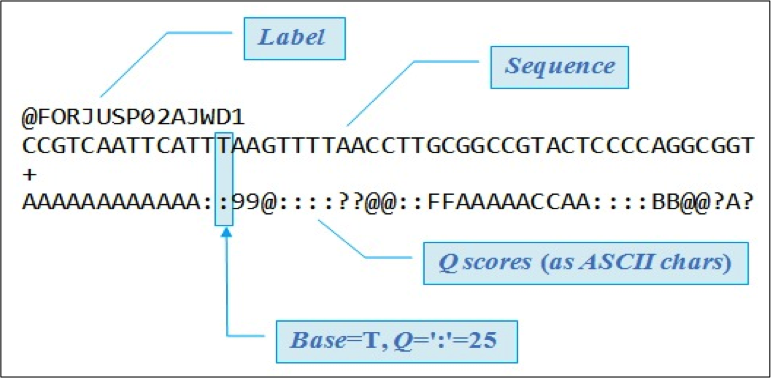
\includegraphics[width=.6\textwidth, height=.3\textwidth]{Fastq_1.png}
    \caption*{Fasq format}
    \label{fastq_1}
\end{figure}
\end{itemize}
The following table describes the elements of Line 1 (See Table \ref{fastq_format})
\scriptsize
\begin{verbatim}
@<instrument>:<run number>:<flowcell ID>:<lane>:<tile>:<x-pos>:<y-pos> <read>:<is filtered>:<control number>: <sample number>
\end{verbatim}
\normalsize

\begin{table}[ht!]
\caption {Fastq Format- Sequence identifier} \label{fastq_format}
\centering
\scalebox{0.8}{
\begin{tabular}{|l|l|l|}
\hline
Element          & Requirements       & Description\\ \hline\hline
@                & @                  & Each sequence identifier line starts with @ \\ \hline
$<\mbox{instrument}>$    & Characters allowed: & Instrument ID \\
                 & a-z, A-Z, 0-9 and  & \\
                 & underscore         & \\ \hline
$<\mbox{run number}>$     & Numerical          & \\ \hline
$<\mbox{flowcell ID}>$    & Characters allowed: & Run number on instrument\\ 
                 & a-z, A-Z, 0-9        & \\ \hline
$<\mbox{lane}>$          & Numerical   & Lane number\\ \hline
$<\mbox{tile}>$          & Numerical   & Tile number \\ \hline
$<\mbox{x\_pos}>$       & Numerical X & Coordinate of cluster  \\ \hline
$<\mbox{y\_pos}>$         & Numerical Y & Coordinate of cluster  \\ \hline
$<\mbox{read}>$         & Numerical   & Read number. 1 can be single read or Read 2 of paired-end  \\ \hline
$<\mbox{is filtered}>$    & Y or N      & Y if the read is filtered (did not pass), N otherwise  \\ \hline
$<\mbox{control number}>$ & Numerical   & 0 when none of the control bits are on, otherwise it is an even number. \\
                 &             & On HiSeq X and NextSeq systems, control specification is not performed and this number is always 0. \\ \hline
$<\mbox{sample number}>$ & Numerical   & Sample number from sample sheet \\ \hline
\end{tabular}}
\end{table}

\section{Trimmomatic}
% Trimmomatic is a lightweight and multithreaded command line java tool application that can be used to
% trim and crop Illumina FASTQ data as well as to remove Illumina adapter sequences and low quality reads.
% It can be used to performs a variety of useful trimming tasks for illumina paired-end and single end mode.
% For single-ended data, one input and one output file are specified, plus the processing steps. For paired-end data,
% two input files are specified, and 4 output files, 2 for the paired output where both reads survived the processing,
% and 2 for corresponding unpaired output where a read survived, but the partner read did not.
% Trimommatic works with FASTQ files (using phred + 33 or phred + 64 quality scores, depending on the Illumina pipeline used).
% It uses a sliding window to analyze chunks of each read, examining the quality score, minimum read length, if it corresponds to an adapter sequence, etc. 
% Files compressed such as gzip or bzip2 are supported, and are identified by use of .gz or .bz2 file extensions.

Trimmomatic is a lightweight and multithreaded command line java tool application that can be used to
\begin{itemize}
 \item To trim and crop Illumina FASTQ data.
 \item To remove Illumina adapter sequences and low quality reads.
 \item To performs a variety of useful trimming tasks for illumina paired-end and single end mode.
For single-ended data, one input and one output file are specified, plus the processing steps. For paired-end data,
two input files are specified, and 4 output files, 2 for the \verb+paired+ output where both reads survived the processing,
and 2 for corresponding \verb+unpaired+ output where a read survived, but the partner read did not.
 \item It works with FASTQ files (using phred + 33 or phred + 64 quality scores, depending on the Illumina pipeline used).
 \item It uses a sliding window to analyze chunks of each read, examining the quality score, minimum read length, if it corresponds to an adapter sequence, etc. 
 \item Files compressed such as \verb+gzip+ or \verb+bzip2+ are supported, and are identified by use of \verb+.gz+ or \verb+.bz2+ file extensions.
\end{itemize}
The selection of trimming steps and their associated parameters are supplied on the command line.
\begin{itemize}
\item ILLUMINACLIP: Cut adapter and other illumina-specific sequences from the read.
\item SLIDINGWINDOW: Perform a sliding window trimming, cutting once the average quality within the window falls below a threshold.
\item LEADING: Cut bases off the start of a read, if below a threshold quality
\item TRAILING: Cut bases off the end of a read, if below a threshold quality
\item CROP: Cut the read to a specified length
\item HEADCROP: Cut the specified number of bases from the start of the read
\item MINLEN: Drop the read if it is below a specified length
\item TOPHRED33: Convert quality scores to Phred-33
\item TOPHRED64: Convert quality scores to Phred-64
\end{itemize}

\section{Install Trimmmomatic}
% \subsection{Install Trimmomatic No recommemded}
% \tiny
% \begin{verbatim}
% $ sudo apt-get install trimmomatic
% 
% [sudo] password for henry: 
% Reading package lists... Done
% Building dependency tree       
% Reading state information... Done
% The following package was automatically installed and is no longer required:
%   libcloog-isl4
% Use 'sudo apt autoremove' to remove it.
% The following additional packages will be installed:
%   libjbzip2-java
% The following NEW packages will be installed:
%   libjbzip2-java trimmomatic
% 0 upgraded, 2 newly installed, 0 to remove and 26 not upgraded.
% Need to get 154 kB of archives.
% After this operation, 241 kB of additional disk space will be used.
% Do you want to continue? [Y/n] y
% Get:1 http://us.archive.ubuntu.com/ubuntu xenial/universe amd64 libjbzip2-java all 0.9.1-3 [39.9 kB]
% Get:2 http://us.archive.ubuntu.com/ubuntu xenial/universe amd64 trimmomatic all 0.35+dfsg-1 [114 kB]
% Fetched 154 kB in 0s (351 kB/s)      
% Selecting previously unselected package libjbzip2-java.
% (Reading database ... 374689 files and directories currently installed.)
% Preparing to unpack .../libjbzip2-java_0.9.1-3_all.deb ...
% Unpacking libjbzip2-java (0.9.1-3) ...
% Selecting previously unselected package trimmomatic.
% Preparing to unpack .../trimmomatic_0.35+dfsg-1_all.deb ...
% Unpacking trimmomatic (0.35+dfsg-1) ...
% Processing triggers for man-db (2.7.5-1) ...
% Setting up libjbzip2-java (0.9.1-3) ...
% Setting up trimmomatic (0.35+dfsg-1) ...
% \end{verbatim}
% \normalsize

\begin{itemize}
\item Download \verb+trimmomatic_0.38+
\scriptsize  
\begin{verbatim}
$ wget http://www.usadellab.org/cms/uploads/supplementary/Trimmomatic/Trimmomatic-Src-0.38.zip
\end{verbatim}
\normalsize
\item Extract the zip file
\scriptsize 
\begin{verbatim}
$ unzip Trimmomatic-Src-0.38.zip
\end{verbatim}
\normalsize
\item Rename the folder as \verb+TRIMHOME+ 
\scriptsize 
\begin{verbatim}
$ mv Trimmomatic-Src-0.38 TRIMHOME

$ cd TRIMHOME
\end{verbatim}
\normalsize
\item Show the folder
\tiny
\begin{verbatim}
henry@Lola:~/TRIMHOME$ tree -d
.
|-- adapters
|-- classes
│    |-- demo
│    |-- META-INF
│    |-- org
│        |-- itadaki
│        │    |-- bzip2
│        |-- usadellab
│            |-- trimmomatic
│                |-- fasta
│                |-- fastq
│                |-- threading
│                |-- trim
│                |-- util
|-- data
│    |-- paired_end
│    |-- single_end
|-- distSrc
|-- lib
|-- src
    |-- org
        |-- usadellab
            |-- trimmomatic
                |-- fasta
                |-- fastq
                |-- threading
                |-- trim
                |-- util

28 directories
\end{verbatim}
\normalsize
\item TREE \verb+TRIMHOME/adapters/+
\tiny
\begin{verbatim}
henry@Lola:~/TRIMHOME$ tree adapters
adapters
|-- NexteraPE-PE.fa
|-- TruSeq2-PE.fa
|-- TruSeq2-SE.fa
|-- TruSeq3-PE-2.fa
|-- TruSeq3-PE.fa
|-- TruSeq3-SE.fa
\end{verbatim}
\normalsize
\item Check if you are really the superuser
\scriptsize 
\begin{verbatim}
henry@Lola:~$ $ whoami
henry
\end{verbatim}
\normalsize
\item The makefile will build 
\begin{enumerate}
\item The \verb+java jar+ file \verb+trimmmomatic.jar+, 
\item The \verb+TRIMHOME/classes+ folder
\item Copy all remain folders from \verb+TRIMHOME+
\end{enumerate}
Use the following  makefile to help you with the installation.
\item Makefile
\tiny
\begin{verbatim}
# http://semver.org/
VERSION := 0.38.0
INSTALL := ${HOME}   # /home/henry
SOURCES := $(shell find src/ -name "*.java" | sed 's|src/||g')

all:
	rm -rf classes; mkdir -p classes/; \
	cd src/; javac -classpath ".:../lib/jbzip2-0.9.jar" -d ../classes ${SOURCES}; \
	cd ../classes; jar xf ../lib/jbzip2-0.9.jar; \
	jar cmf ../MANIFEST.MF trimmomatic.jar ./

check:
	@echo "this package doesn't have any test (yet)"

install: 
	mkdir -p ${INSTALL}/TRIMHOME                       # Created folder /home/henry/TRIMHOME 
	cp classes/trimmomatic.jar ${INSTALL}/TRIMHOME/    # Copy  classes/trimmomatic.jar into  /home/henry/TRIMHOME/trimmomatic.jar
	cp -vrf * ${INSTALL}/TRIMHOME/                     # Copy  all filestrimmomatic-038

dist:
	mkdir -p trimmomatic-${VERSION}
	cp AUTHORS Makefile README trimmomatic-${VERSION}
	cp build.xml MANIFEST.MF versionHistory.txt trimmomatic-${VERSION}
	cp -r adapters distSrc lib/ src/ trimmomatic-${VERSION}
	tar -czvf trimmomatic-${VERSION}.tar.gz trimmomatic-${VERSION}/
	rm -rf trimmomatic-${VERSION}

clean:
	rm -rf classes/
\end{verbatim}
\normalsize
\item Use Makefile
\begin{enumerate}
\item Install \verb+trimmomatic-0.38+ packages without know where (No recommemded)
\scriptsize 
\begin{verbatim}
henry@Lola:~$ cd trimmomatic-0.38
\end{verbatim}
\normalsize
% \tiny
% \begin{verbatim}
% henry@Lola:~$ cd trimmomatic-0.38
% henry@Lola:~/trimmomatic-0.38$ ll
% total 68
% drwxr-xr-x  8 henry henry 4096 Oct 24 13:59 ./
% drwxrwxr-x 13 henry henry 4096 Oct 23 09:06 ../
% drwxr-xr-x  2 henry henry 4096 May 16 09:06 adapters/
% -rw-rw-r--  1 henry henry   84 Mar 10  2015 AUTHORS
% -rw-r--r--  1 henry henry 2689 May 16 09:06 build.xml
% drwxrwxr-x  5 henry henry 4096 Oct 24 12:16 classes/
% drwxr-xr-x  2 henry henry 4096 May 16 09:06 distSrc/
% drwxr-xr-x  2 henry henry 4096 May 16 09:06 lib/
% -rwxrwxrwx  1 henry henry 1009 Oct 24 13:59 Makefile*
% -rw-r--r--  1 henry henry   50 May 16 09:06 MANIFEST.MF
% -rw-rw-r--  1 henry henry  744 Mar 10  2015 README
% drwxr-xr-x  3 henry henry 4096 May 16 09:06 src/
% drwxr-xr-x  2 root  root  4096 Oct 24 13:47 TRIMHOME/
% -rw-r--r--  1 henry henry  540 May 16 09:06 versionHistory.txt
% \end{verbatim}
% \normalsize
\scriptsize 
\begin{verbatim}
henry@Lola:~/trimmomatic-0.38$  make install
\end{verbatim}
\normalsize
\begin{itemize}
 \item Find \verb+$HOME+, 
\scriptsize 
\begin{verbatim}
henry@Lola:~$ $HOME
bash: /home/henry: Is a directory
\end{verbatim}
\normalsize
\item Find where was installed
\scriptsize 
\begin{verbatim}
henry@Lola:~/TRIMHOME$ pwd
/home/henry/TRIMHOME
\end{verbatim}
\normalsize
\end{itemize}
\item Install \verb+trimmomatic-0.38+ packages on a specific location
\begin{itemize}
\item Where 
\scriptsize 
\begin{verbatim}
/usr/local/TRIMHOME/
\end{verbatim}
\normalsize
\item How we installed the trimmomatic packages
\scriptsize  
\begin{verbatim}
make
make check
make install INSTALL="/usr/local/"
\end{verbatim}
\normalsize
\end{itemize}
\end{enumerate}
\item TREE data
\tiny
\begin{verbatim}
henry@Lola:~/data$ tree data
data
|
|-- paired_end
│    |-- ERR950159_1.fastq
│    |-- ERR950159_2.fastq
│    |-- ERR950173_1.fastq
│    |-- ERR950173_2.fastq
│    |-- ERR950179_1.fastq
│    |-- ERR950179_2.fastq
|
|-- single_end
    |-- ERR458493.fastq
    |-- ERR458493.fastq.gz
    |-- ERR458494.fastq.gz
    |-- ERR458495.fastq.gz
    |-- SRR020192.fastq.gz
    |-- yeast_data.tar.gz
\end{verbatim}
\normalsize
\end{itemize}

\section{How Trimmomatic Work}
\begin{itemize}
\item Trimmomatic is a program written in the Java programming language. 
\begin{enumerate}
\item Check your Java version
\scriptsize  
\begin{verbatim}
$ java -version
openjdk version "1.8.0_131"
OpenJDK Runtime Environment (build 1.8.0_131-8u131-b11-0ubuntu1.16.04.2-b11)
OpenJDK 64-Bit Server VM (build 25.131-b11, mixed mode)
\end{verbatim}
\normalsize
or
\scriptsize  
\begin{verbatim}
$ javac -version
javac 1.8.0_131
\end{verbatim}
\normalsize
\end{enumerate}
\item Input files (single end and paired end)
 \tiny 
\begin{verbatim}
henry@Lola:~/TRIMHOME$$ tree data
data
|
|-- paired_end
│    |-- ERR950159_1.fastq
│    |-- ERR950159_2.fastq
│    |-- ERR950173_1.fastq
│    |-- ERR950173_2.fastq
│    |-- ERR950179_1.fastq
│    |-- ERR950179_2.fastq
|
|-- single_end
    |-- ERR458493.fastq
    |-- ERR458493.fastq.gz
    |-- ERR458494.fastq.gz
    |-- ERR458495.fastq.gz
    |-- SRR020192.fastq.gz
    |-- yeast_data.tar.gz

2 directories, 23 files
\end{verbatim}
\normalsize
\item Output files
 \tiny 
\begin{verbatim}
henry@Lola:~/TRIMHOME$$ tree data
data
|
|-- paired_end
│    |-- output_forward_paired_ERR950159_1.fastq
│    |-- output_forward_unpaired_ERR950159_1.fastq
│    |-- output_reverse_paired_ERR950159_2.fastq
│    |-- output_reverse_unpaired_ERR950159_2.fastq
|
|-- single_end
    |-- OUT_ERR458493.fastq


2 directories, 23 files
\end{verbatim}
\normalsize
\item The complete command for Trimmomatic
\begin{enumerate}
\item  HOME
\scriptsize  
\begin{verbatim}
$ $HOME
bash: /home/henry: Is a directory
\end{verbatim}
\normalsize
 \item Single end
 \tiny 
\begin{verbatim}
$ java -jar /usr/local/TRIMHOME/trimmomatic.jar SE -threads 4 -phred33  
~/Desktop/RNA_Seq_Differential_Expressions/FASTQ_Files/single_end/ERR458493.fastq
~/Desktop/RNA_Seq_Differential_Expressions/FASTQ_Files/single_end/OUT_ERR458493.fastq  
ILLUMINACLIP:/usr/local/TRIMHOME/adapters/TruSeq3-SE.fa:2:30:10 LEADING:3 TRAILING:3 SLIDINGWINDOW:4:15 MINLEN:36

TrimmomaticSE: Started with arguments:
 -threads 4 -phred33 /home/henry/Desktop/RNA_Seq_Differential_Expressions/FASTQ_Files/single_end/ERR458493.fastq 
 /home/henry/Desktop/RNA_Seq_Differential_Expressions/FASTQ_Files/single_end/OUT_ERR458493.fastq 
 ILLUMINACLIP:/usr/local/TRIMHOME/adapters/TruSeq3-SE.fa:2:30:10 LEADING:3 TRAILING:3 SLIDINGWINDOW:4:15 MINLEN:36
Using Long Clipping Sequence: 'AGATCGGAAGAGCGTCGTGTAGGGAAAGAGTGTA'
Using Long Clipping Sequence: 'AGATCGGAAGAGCACACGTCTGAACTCCAGTCAC'
ILLUMINACLIP: Using 0 prefix pairs, 2 forward/reverse sequences, 0 forward only sequences, 0 reverse only sequences
Input Reads: 1093957 Surviving: 1073395 (98.12%) Dropped: 20562 (1.88%)
TrimmomaticSE: Completed successfully
\end{verbatim}
\normalsize
 \item Paired end
 \tiny 
\begin{verbatim}
$ java -jar /usr/local/TRIMHOME/trimmomatic.jar PE -threads 12 -phred33 
~/Desktop/RNA_Seq_Differential_Expressions/FASTQ_Files/paired_end/ERR950159_1.fastq 
~/Desktop/RNA_Seq_Differential_Expressions/FASTQ_Files/paired_end/ERR950159_2.fastq  
~/Desktop/RNA_Seq_Differential_Expressions/FASTQ_Files/paired_end/output_forward_paired_ERR950159_1.fastq 
~/Desktop/RNA_Seq_Differential_Expressions/FASTQ_Files/paired_end/output_forward_unpaired_ERR950159_1.fastq 
~/Desktop/RNA_Seq_Differential_Expressions/FASTQ_Files/paired_end/output_reverse_paired_ERR950159_2.fastq  
~/Desktop/RNA_Seq_Differential_Expressions/FASTQ_Files/paired_end/output_reverse_unpaired_ERR950159_2.fastq 
ILLUMINACLIP:/usr/local/TRIMHOME/adapters/TruSeq3-PE.fa:2:30:10 LEADING:3 TRAILING:3 SLIDINGWINDOW:4:15 MINLEN:36

TrimmomaticPE: Started with arguments:
 -threads 12 -phred33 /home/henry/Desktop/RNA_Seq_Differential_Expressions/FASTQ_Files/paired_end/ERR950159_1.fastq
 /home/henry/Desktop/RNA_Seq_Differential_Expressions/FASTQ_Files/paired_end/ERR950159_2.fastq 
 /home/henry/Desktop/RNA_Seq_Differential_Expressions/FASTQ_Files/paired_end/output_forward_paired_ERR950159_1.fastq 
 /home/henry/Desktop/RNA_Seq_Differential_Expressions/FASTQ_Files/paired_end/output_forward_unpaired_ERR950159_1.fastq 
 /home/henry/Desktop/RNA_Seq_Differential_Expressions/FASTQ_Files/paired_end/output_reverse_paired_ERR950159_2.fastq
 /home/henry/Desktop/RNA_Seq_Differential_Expressions/FASTQ_Files/paired_end/output_reverse_unpaired_ERR950159_2.fastq 
 ILLUMINACLIP:/usr/local/TRIMHOME/adapters/TruSeq3-PE.fa:2:30:10 LEADING:3 TRAILING:3 SLIDINGWINDOW:4:15 MINLEN:36
Using PrefixPair: 'TACACTCTTTCCCTACACGACGCTCTTCCGATCT' and 'GTGACTGGAGTTCAGACGTGTGCTCTTCCGATCT'
ILLUMINACLIP: Using 1 prefix pairs, 0 forward/reverse sequences, 0 forward only sequences, 0 reverse only sequences
Input Read Pairs: 21433074 Both Surviving: 17241380 (80.44%) Forward Only Surviving: 3912653 (18.26%) Reverse Only Surviving: 143989 (0.67%) Dropped: 135052 (0.63%)
TrimmomaticPE: Completed successfully
\end{verbatim}
\normalsize
\end{enumerate}
\item Let break the command to run Trimmomatic 
\begin{enumerate}
 \item Trimommatic starts with 
 \scriptsize  
\begin{verbatim}
$ java -jar /path_to_the_java_jar/trimmomatic.jar
\end{verbatim}
\normalsize
\begin{itemize}
 \item \verb+java+ tells our computer that we’re running a Java program. 
 \item \verb+-jar+ is an option specifying that we’re going to specify the location of the Java program we want to run
 \item \verb+/path_to_the_java_jar/trimmomatic.jar+ is the java executable tool.
\end{itemize}
\item Trimommatic attributes
\begin{itemize}
 \item \verb+PE+
 \item \verb+-threads 12+
 \item \verb+-phred33+
\end{itemize}
\item Input file
\begin{enumerate}
 \item Single end
 \tiny 
\begin{verbatim}
~/Desktop/RNA_Seq_Differential_Expressions/FASTQ_Files/single_end/ERR458493.fastq
\end{verbatim}
\normalsize
 \item Paired end
 \tiny 
\begin{verbatim}
~/Desktop/RNA_Seq_Differential_Expressions/FASTQ_Files/paired_end/ERR950159_1.fastq 
~/Desktop/RNA_Seq_Differential_Expressions/FASTQ_Files/paired_end/ERR950159_2.fastq  
\end{verbatim}
\normalsize
\end{enumerate}
\item Output Files
\begin{enumerate}
 \item Single end
 \tiny 
\begin{verbatim}
~/Desktop/RNA_Seq_Differential_Expressions/FASTQ_Files/single_end/OUT_ERR458493.fastq  
\end{verbatim}
\normalsize
 \item Paired end
 \tiny 
\begin{verbatim}
~/Desktop/RNA_Seq_Differential_Expressions/FASTQ_Files/paired_end/output_forward_paired_ERR950159_1.fastq 
~/Desktop/RNA_Seq_Differential_Expressions/FASTQ_Files/paired_end/output_forward_unpaired_ERR950159_1.fastq 
~/Desktop/RNA_Seq_Differential_Expressions/FASTQ_Files/paired_end/output_reverse_paired_ERR950159_2.fastq  
~/Desktop/RNA_Seq_Differential_Expressions/FASTQ_Files/paired_end/output_reverse_unpaired_ERR950159_2.fastq 
\end{verbatim}
\normalsize
\end{enumerate}
\item ILLUMINA Attributes
\begin{enumerate}
 \item Single end
 \tiny 
\begin{verbatim}
ILLUMINACLIP:/usr/local/TRIMHOME/adapters/TruSeq3-SE.fa:2:30:10 LEADING:3 TRAILING:3 SLIDINGWINDOW:4:15 MINLEN:36
\end{verbatim}
\normalsize
 \item Paired end
 \tiny 
\begin{verbatim}
ILLUMINACLIP:/usr/local/TRIMHOME/adapters/TruSeq3-PE.fa:2:30:10 LEADING:3 TRAILING:3 SLIDINGWINDOW:4:15 MINLEN:36
\end{verbatim}
\normalsize
\end{enumerate}
\end{itemize}
\end{itemize}


\section{Python code to execute trimmmomatic}
\begin{itemize}
\item Example 1:
\tiny  
\begin{verbatim}
# Load modules
from Bio import SeqIO  # module needed for sequence input  
import sys             # module needed for command line argument to get fastq name  
import re              # module for Regular expression operations, this module provides regular expression matching operations similar to those found in Perl.
import os

# Compiler and path tool
ja = " java -jar"
tool = " /usr/local/TRIMHOME/trimmomatic.jar"
s = " "
# Execute Single end or Paired end
mode = raw_input("Please enter enter mode (Single [1]  or Paired [2]): ")
print 'Mode = ', mode

if mode == 'Single' or mode == '1':  
   print "Sigle End mode : Supply fastq file\n"
   # Load data 
   file_input = "/home/henry/Desktop/RNA_Seq_Differential_Expressions/FASTQ_Files/single_end/ERR458493.fastq"
   fastqfile1 = open(file_input, 'r') 
   # Output single end
   file_output = "/home/henry/Desktop/RNA_Seq_Differential_Expressions/FASTQ_Files/single_end/output_single_ERR458493.fastq"
   # FASTQ file where you want to trim all the reads
   count = 0
   for rec in SeqIO.parse(fastqfile1, "fastq"):
      count += 1
   print("farsq %i reads\n" % count)   # count reads

   print "Start Trimmonatics :"    #java -jar trimmomatic SE -threads 4 -phred33 file_input file_output ILLUMINACLIP:adapters:2:30:10 LEADING:3 TRAILING:3 SLIDINGWINDOW:4:15 MINLEN:36
   print "--------------------" 
   attribute              = " SE -threads 4 -phred33"
   illuminaclip_adapters  = "ILLUMINACLIP:/usr/local/TRIMHOME/adapters/TruSeq3-SE.fa:2:30:10"
   illuminaclip_Attribute = "LEADING:3 TRAILING:3 SLIDINGWINDOW:4:15 MINLEN:36"
   cmd  = s + ja + s + tool + s + attribute + s + file_input + s + file_output + s + illuminaclip_adapters + s + illuminaclip_Attribute
   os.system(cmd)

elif mode == 'Paired' or mode == '2': 
   print "Paired End mode: Supply a forward and reverse fastq files\n"
# Load data forward
   filename_forward = "/home/henry/Desktop/RNA_Seq_Differential_Expressions/FASTQ_Files/paired_end/ERR950159_1.fastq"
   fastq_forward = open(filename_forward, 'r')  # Here you write your fastq filename
   # FASTQ file where you want to trim all the reads
   #count = 0
   #for rec in SeqIO.parse(fastq_forward, "fastq"):
   #   count += 1
   #print("fastq forward %i reads" % count)   # count reads

   # Load data reverse
   filename_reverse = "/home/henry/Desktop/RNA_Seq_Differential_Expressions/FASTQ_Files/paired_end/ERR950159_2.fastq"
   fastq_reverse = open(filename_reverse, 'r') 
   # FASTQ file where you want to trim all the reads
   #count = 0
   #for rec in SeqIO.parse(fastq_reverse, "fastq"):
   #   count += 1
   #print("fastq reverse %i reads" % count)   # count reads

   # Outputs paired end
   output_forward_paired = "/home/henry/Desktop/RNA_Seq_Differential_Expressions/FASTQ_Files/paired_end/output_forward_paired_ERR950159_1.fastq" 
   output_forward_unpaired = "/home/henry/Desktop/RNA_Seq_Differential_Expressions/FASTQ_Files/paired_end/output_forward_unpaired_ERR950159_1.fastq" 
   output_reverse_paired = "/home/henry/Desktop/RNA_Seq_Differential_Expressions/FASTQ_Files/paired_end/output_reverse_paired_ERR950159_2.fastq"  
   output_reverse_unpaired = "/home/henry/Desktop/RNA_Seq_Differential_Expressions/FASTQ_Files/paired_end/output_reverse_unpaired_ERR950159_2.fastq" 

   print "Start Trimmonatics :"    
   print "--------------------" 
   attribute              = "PE -threads 12 -phred33 "
   illuminaclip_adapters  = "ILLUMINACLIP:/usr/local/TRIMHOME/adapters/TruSeq3-PE.fa:2:30:10"
   illuminaclip_Attribute = "LEADING:3 TRAILING:3 SLIDINGWINDOW:4:15 MINLEN:36"
   cmd1 = s + ja + s + tool + s + attribute + s + filename_forward + s + filename_reverse + s + output_forward_paired + s + output_forward_unpaired
   cmd2 = s + output_reverse_paired + s + output_reverse_unpaired + s + illuminaclip_adapters + s + illuminaclip_Attribute
   cmd  =  cmd1 + cmd2
   os.system(cmd)
\end{verbatim}
\normalsize
\item Example 2:
\tiny  
\begin{verbatim}
# Load modules
from Bio import SeqIO  # module needed for sequence input  
import sys             # module needed for command line argument to get fastq name  
import re              # module for Regular expression operations, this module provides regular expression matching operations similar to those found in Perl.
import subprocess

# Compiler and path tool
ja = " java -jar"
tool = " /usr/local/TRIMHOME/trimmomatic.jar"
s = " "
# Execute Single end or Paired end
mode = raw_input("Please enter enter mode (Single [1]  or Paired [2]): ")
print 'Mode = ', mode

if mode == 'Single' or mode == '1':  
   print "Sigle End mode : Supply fastq file\n"
   # Load data 
   file_input = "/home/henry/Desktop/RNA_Seq_Differential_Expressions/FASTQ_Files/single_end/ERR458493.fastq"
   fastqfile1 = open(file_input, 'r') 
   # Output single end
   file_output = "/home/henry/Desktop/RNA_Seq_Differential_Expressions/FASTQ_Files/single_end/output_single_ERR458493.fastq"
   # FASTQ file where you want to trim all the reads
   count = 0
   for rec in SeqIO.parse(fastqfile1, "fastq"):
      count += 1
   print("farsq %i reads\n" % count)   # count reads

   print "Start Trimmonatics :"    #java -jar trimmomatic SE -threads 4 -phred33 file_input file_output ILLUMINACLIP:adapters:2:30:10 LEADING:3 TRAILING:3 SLIDINGWINDOW:4:15 MINLEN:36
   print "--------------------" 
   attribute              = " SE -threads 4 -phred33"
   illuminaclip_adapters  = "ILLUMINACLIP:/usr/local/TRIMHOME/adapters/TruSeq3-SE.fa:2:30:10"
   illuminaclip_Attribute = "LEADING:3 TRAILING:3 SLIDINGWINDOW:4:15 MINLEN:36"
   cmd  = s + ja + s + tool + s + attribute + s + file_input + s + file_output + s + illuminaclip_adapters + s + illuminaclip_Attribute
   call = ["/bin/bash", "-c", cmd]
   ret  = subprocess.call(call, stdout=None, stderr=None)
   if ret > 0:
      print "Warning - result was %d" % ret

elif mode == 'Paired' or mode == '2': 
   print "Paired End mode: Supply a forward and reverse fastq files\n"
# Load data forward
   filename_forward = "/home/henry/Desktop/RNA_Seq_Differential_Expressions/FASTQ_Files/paired_end/ERR950159_1.fastq"
   fastq_forward = open(filename_forward, 'r')  # Here you write your fastq filename
   # FASTQ file where you want to trim all the reads
   #count = 0
   #for rec in SeqIO.parse(fastq_forward, "fastq"):
   #   count += 1
   #print("fastq forward %i reads" % count)   # count reads

   # Load data reverse
   filename_reverse = "/home/henry/Desktop/RNA_Seq_Differential_Expressions/FASTQ_Files/paired_end/ERR950159_2.fastq"
   fastq_reverse = open(filename_reverse, 'r') 
   # FASTQ file where you want to trim all the reads
   #count = 0
   #for rec in SeqIO.parse(fastq_reverse, "fastq"):
   #   count += 1
   #print("fastq reverse %i reads" % count)   # count reads

   # Outputs paired end
   output_forward_paired = "/home/henry/Desktop/RNA_Seq_Differential_Expressions/FASTQ_Files/paired_end/output_forward_paired_ERR950159_1.fastq" 
   output_forward_unpaired = "/home/henry/Desktop/RNA_Seq_Differential_Expressions/FASTQ_Files/paired_end/output_forward_unpaired_ERR950159_1.fastq" 
   output_reverse_paired = "/home/henry/Desktop/RNA_Seq_Differential_Expressions/FASTQ_Files/paired_end/output_reverse_paired_ERR950159_2.fastq"  
   output_reverse_unpaired = "/home/henry/Desktop/RNA_Seq_Differential_Expressions/FASTQ_Files/paired_end/output_reverse_unpaired_ERR950159_2.fastq" 

   print "Start Trimmonatics :"    
   print "--------------------" 
   attribute              = "PE -threads 12 -phred33 "
   illuminaclip_adapters  = "ILLUMINACLIP:/usr/local/TRIMHOME/adapters/TruSeq3-PE.fa:2:30:10"
   illuminaclip_Attribute = "LEADING:3 TRAILING:3 SLIDINGWINDOW:4:15 MINLEN:36"
   cmd1 = s + ja + s + tool + s + attribute + s + filename_forward + s + filename_reverse + s + output_forward_paired + s + output_forward_unpaired
   cmd2 = s + output_reverse_paired + s + output_reverse_unpaired + s + illuminaclip_adapters + s + illuminaclip_Attribute
   cmd  =  cmd1 + cmd2
   call = ["/bin/bash", "-c", cmd]
   ret  = subprocess.call(call, stdout=None, stderr=None)
   if ret > 0:
      print "Warning - result was %d" % ret
\end{verbatim}
\normalsize
\end{itemize}

% \section{Building Pipeline Examples}
% \subsection{Example 1}
% \scriptsize
% \begin{verbatim}
%    
% \end{verbatim}
% \normalsize
% 
% \subsection{Example 2}
% \scriptsize
% \begin{verbatim}
%    
% \end{verbatim}
% \normalsize



% 
% \section{Requiere Software}
% \cite{Aladin_2014_Yakun_Shopia}.
% \cite{SV_Periodic_Structures_in_Electromagnetic_2015})
% \cite{petsc_web_page}, \cite{FFTW})
% \begin{figure}[htp]
%     \centering
%     \includegraphics[width=.8\textwidth, height=.4\textwidth]{petsc_3_5_4_with_fftw_and_complex_number_configuration.eps}
%     \caption*{PetscScalar: Evaluate the Computer System using Complex Numbers}
%     \label{checkerboard_lattice}
% \end{figure}

%%%%%%%%%%%%%%%%%%%%%%%%%%%%%%%%%%%%%%%%%%%%%%%%%%%%%%%%%%%%%%%%%%%%%%%%%%%%%%%%
                        % Concluding Pages %
%%%%%%%%%%%%%%%%%%%%%%%%%%%%%%%%%%%%%%%%%%%%%%%%%%%%%%%%%%%%%%%%%%%%%%%%%%%%%%%%



%%%%%%%%%%%%%%%%%%%%%%%%%%%%%%%%%%%%%%%%%%%%%%%%%%%%%%%%%%%%%%%%%%%%%%%%%%%%%%%%
                             % Appendices Pages %
%%%%%%%%%%%%%%%%%%%%%%%%%%%%%%%%%%%%%%%%%%%%%%%%%%%%%%%%%%%%%%%%%%%%%%%%%%%%%%%%

% \appendix
% \section{Appendices}
% \subsection{First appendix}
% \subsection{Second appendix}

% \appendix
% \addcontentsline{toc}{section}{Appendices}
% \section*{Appendices}
% \section{First appendix}
% \section{Second appendix}


%%%%%%%%%%%%%%%%%%%%%%%%%%%%%%%%%%%%%%%%%%%%%%%%%%%%%%%%%%%%%%%%%%%%%%%%%%%%%%%%
                           %  Bibliography Pages %
%%%%%%%%%%%%%%%%%%%%%%%%%%%%%%%%%%%%%%%%%%%%%%%%%%%%%%%%%%%%%%%%%%%%%%%%%%%%%%%%

% Bibliography or References, REQUIRED

% If using bibtex, create or modify the refs.bib file
% and use (uncomment) the following three lines.
%\bibliographystyle{plain}     %You may prefer \bibliographystyle{alpha}
%\addcontentsline{toc}{chapter}{\bibname}
%\bibliography{refs}         

% If using the ``thereference'' environment instead, modify the ref.tex file
% and use the following line
%\include{ref}
%\bibliography{Bibliography_HTCondor}
\newpage
\bibliography{References/TOOLS_Bibliography}
\end{document}
